\documentclass[a4paper,12pt]{article}

\usepackage[T2A]{fontenc}
\usepackage[utf8]{inputenc}
\usepackage[english,russian]{babel}
\usepackage{amsmath}
\usepackage{geometry}
\usepackage{graphicx}
\usepackage[section,above,below]{placeins}
\usepackage{afterpage,placeins}
\usepackage{booktabs}
\usepackage{caption}

\usepackage{algorithm}
\usepackage[noend]{algpseudocode}

\DeclareGraphicsExtensions{.png,.jpg}

\geometry{left=2cm}
\geometry{right=1.5cm}
\geometry{top=1cm}
\geometry{bottom=1.5cm}

\headheight = 1cm
\footskip = 0pt
%\usepackage[left=20mm, top=10mm, right=10mm, bottom=5mm, nohead, nofoot]{geometry}

\parskip = 4.25mm % расстояние между строками
\parindent=6.375mm % расстояние между абзацами
\floatname{algorithm}{Алгоритм} % переопределение имени в псевдокоде

\usepackage{listings}
\usepackage{color}


\lstset{
	language=Go,
	basicstyle=\ttfamily,
	keywordstyle=\color{blue}\ttfamily,
	stringstyle=\color{red}\ttfamily,
	commentstyle=\color{green}\ttfamily
}

\begin{document}

    \begin{titlepage}

        \begin{center}
            \large
            Государственное образовательное учреждение высшего образования\\
            “Московский государственный технический университет имени Н.Э.Баумана”
            \vspace{3cm}
            
            \textsc{Дисциплина: Анализ алгоритмов}
            \vspace{0.5cm}
                
            \textsc{Лабораторная работа №5}
            \vspace{3cm}
            
            {\LARGE Конвейер}
            \vspace{3cm}
            
            Студент группы ИУ7-54Б,\\   
            Котов Никита
            \vfill
            
            2019 г.
            
            \end{center}
    \end{titlepage}
    
    \begin{center}
    	\tableofcontents
    \end{center}
	
	\setcounter{page}{2}
	\newpage
    \begin{center}
        \section*{Введение}
        \addcontentsline{toc}{section}{Введение}
    \end{center}
        \label{sec:intro}

	При обработке данных могут возникать ситуации, когда необходимо обработать множество данных последовательно несколькими алгоритмами. В этом случае удобно использовать конвейерную обработку данных. Это может быть полезно при следующих задачах:
		\begin{itemize}
		    \item шифровании данных;
   		    \item сортировки и фильтрации данных;
   		    \item и др.
		\end{itemize}  
		
Цель данной работы: получить навык организации асинхронного взаимодействия потоков на примере конвейерной обработки данных.

В рамках выполнения работы необходимо решить следующие задачи:   
		\begin{itemize}
		    \item рассмотреть и изучить конвейерную обработку данных;
			\item реализовать конвейер с количеством лент не меньше трех в многопоточной среде;
			\item на основании проделанной работы сделать выводы.
		\end{itemize}
    \newpage

    \begin{center}
        \section{Аналитическая часть}
	    \subsection{Описание конвейерной обработки данных}
    \end{center}
	
	При конвейерной обработке данных каждая лента имеет свою очередь с некоторыми задачами, ожидающими обработки. Лента берет данные из своей очереди с входными данными, проводит с ними необходимые операции и передает в очередь следующей ленты или, в случае последней ленты, в пул обработанных задач.	
	
    \newpage

    \begin{center}
        \section{Конструкторская часть}
        \subsection{Разработка конвейерной обработки данных}        
    \end{center}
    
	Принцип работы стадийной обработки представлен на рис.~\ref{ris:matr_dl_sh1}.
	\begin{figure}[h]
		 			\centering
		 			{
		 				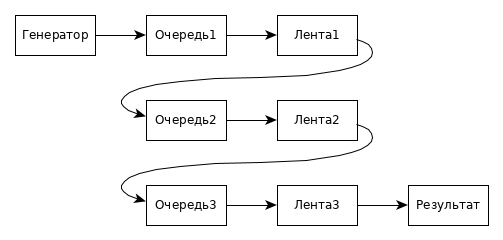
\includegraphics[scale=0.85]{ris.png}
		 				\captionsetup{labelsep=period}
		 				\caption{Конвейерная обработка данных}
		 				\label{ris:matr_dl_sh1}
		 			}
		 		\end{figure}	
    
    \newpage
    \afterpage{\FloatBarrier}
    
    \begin{center}
     	\section{Технологическая часть}
    	\subsection{Требования к программному обеспечению}
    \end{center}
    
    	В программе должны быть реализованы как минимум три ленты обработки данных и обеспечен вывод времени входа и выхода каждой задачи из каждой ленты.
    	
    \begin{center}
    % It won't work without this
    \end{center}
    \begin{center}
        \subsection{Средства реализации}    
    \end{center}
    
		В качестве языка программирования был выбран Golang, так как он предоставляет широкие возможности и крайне удобный интерфейс для эффективной реализации асинхронной, параллельной обработки данных [1].
		
		Для измерения времени использовалась стандартная библиотека time. Так как основное время работы составляет ожидание sleep, то достаточно замерить время работы один раз.

		\newpage
    \begin{center}
        \subsection{Листинг кода}    
    \end{center}		
    
    	В листинге 1 представлена реализация конвейерная обработка данных.		
        	
        		\begin{lstlisting}[frame=single,title=Листинг 1. Конвейерная обработка данных, breaklines]
package main

import (
	"fmt"
	"math/rand"
	"sync"
	"time"
)

const (
	TasksNumber = 3
)

type job func(in, out chan interface{})

type Task struct {
	Value       int
	Result      int
	StartTimes  []time.Time
	EndTimes    []time.Time
}

func startJob(function job, in, out chan interface{}, wg *sync.WaitGroup) {
	defer wg.Done()
	defer close(out)
	function(in, out)
}

func ExecutePipeline(jobs ...job) {
	wg := &sync.WaitGroup{}
	inChan := make(chan interface{}, TasksNumber)

	for _, jobItem := range jobs {
		outChan := make(chan interface{}, TasksNumber)
		wg.Add(1)

		go startJob(jobItem, inChan, outChan, wg)
		inChan = outChan
	}

	wg.Wait()
}

func dataGenerator(_, out chan interface{}) {
	s := rand.NewSource(time.Now().UnixNano())
	r := rand.New(s)
	for i := 0; i < TasksNumber; i++ {
		val := r.Intn(100)
		task := Task{Value: val, Result: val}
		out <- task
	}
}

func makeHandler(sleepDuration int, multiplier int) func(chan interface{}, chan interface{}) {
	return func(in, out chan interface{}) {
		for rawTask := range in {
			task := rawTask.(Task)
			task.StartTimes = append(task.StartTimes, time.Now())

			task.Result *= multiplier
			time.Sleep(time.Millisecond * time.Duration(sleepDuration))

			task.EndTimes = append(task.EndTimes, time.Now())
			out <- task
		}
	}
}

func logHandler(in, _ chan interface{}) {
	for rawTask := range in {
		task := rawTask.(Task)
		fmt.Printf("Task's start value = %d, result = %d\n", task.Value, task.Result)
		fmt.Printf("Start 1st: %s, end 1st: %s\n", task.StartTimes[0].Local(), task.EndTimes[0].Local())
		fmt.Printf("Start 2nd: %s, end 2nd: %s\n", task.StartTimes[1].Local(), task.EndTimes[1].Local())
		fmt.Printf("Start 3d: %s, end 3d: %s\n", task.StartTimes[2].Local(), task.EndTimes[2].Local())
		fmt.Println()
	}
}

func main() {
	jobs := []job{
		job(dataGenerator),
		job(makeHandler(100, 2)),
		job(makeHandler(200, 3)),
		job(makeHandler(300, 2)),
		job(logHandler),
	}

	ExecutePipeline(jobs...)
}

\end{lstlisting}
    \newpage
    \begin{center}
		\subsection{Тестирование фунций}
	\end{center}
	
		Для тестирования были реализованы функции, представленные на листинге 2. Результаты тестирования представоены в таблице~\ref{tabular:test_rec}. Видно, что тестирование пройдено успешно.
\begin{lstlisting}[frame=single,title=Листинг 2. Тестовые задачи, breaklines]
		job(func(in, out chan interface{}) {
			out <- uint32(1)
			out <- uint32(3)
			out <- uint32(4)
		}),
		job(func(in, out chan interface{}) {
			for val := range in {
				out <- val.(uint32) * 3
			}
		}),
		job(func(in, out chan interface{}) {
			for val := range in {
				fmt.Println("collected", val)
				atomic.AddUint32(&recieved, val.(uint32))
			}
		}),
\end{lstlisting}
        			\begin{table}[H]     
        			\captionsetup{labelsep=period}   		
       				\caption{\label{tabular:test_rec} Тестирование конвейерной обработки}
       				\begin{center}       			
        			\begin{tabular}{|c|c|c|}        				
        				\hline
						Входные данные & Ожидаемый результат & Результат \\ 
						\hline
        				1,3,4    & 24  & 24\\
        				\hline
        			\end{tabular}
       				\end{center}
        			\end{table}        			
        		
	\newpage

    \begin{center}
        \section{Экспериментальная часть}
	    \subsection{Замеры времени работы функций}	
	\end{center}
	    
	    Реализованная контейнерная обработка данных работает за 1,2с. Последовательная реализация потребовала бы $(0,1 + 0,2 + 0,3) * 3 = 1,8\text{с}$, что на 50\% медленней.
    \newpage

    \begin{center}
        \section*{Заключение}
        \addcontentsline{toc}{section}{Заключение}
    \end{center}
            \label{sec:ending}
            
            В рамках лабораторной работы была рассмотрена и изучена конвейерная обработка данных. Благодаря ней возможна крайне удобная реализация задач, тербующих поэтапной обработки некоторого набора данных, а также в некоторых случаях позволяет значительно ускорить выполнение программы (в реализованном синтетическом примере выигрыш составил 50\%).
    \newpage


	\addcontentsline{toc}{section}{Список литературы}
    \begin{center}        
        \begin{thebibliography}{}
        	\bibitem{litlink1}  Dan Gorby. Multi-thread For Loops Easily and Safely in Go  [Электронный ресурс]//  Medium.  2016.  8 февраля.  URL:https://medium.com/@greenraccoon23/multi-thread-for-loops-easily-and-safely-in-go-a2e915302f8b (дата обращения: 28.10.2019).   	 	
        	
        \end{thebibliography}
    \end{center}

\end{document}
